\documentclass{article}
\usepackage{amsmath}
\usepackage{amsfonts}
\usepackage{amssymb}
\usepackage{graphicx}
\usepackage{tikz}

\begin{document}

\begin{figure}[h]
    \centering
    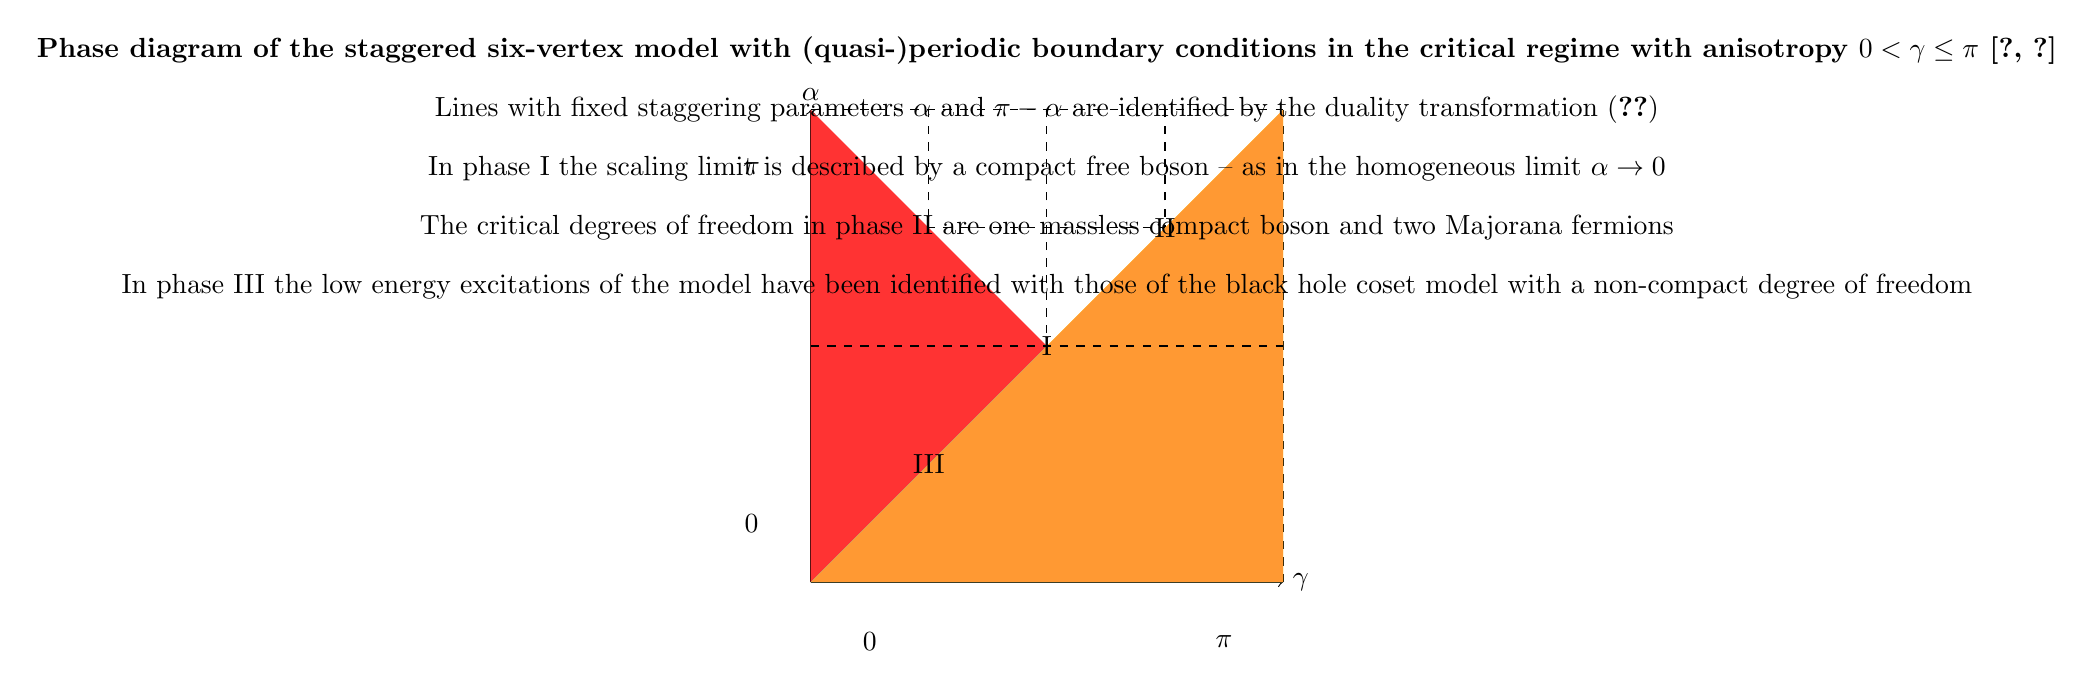
\begin{tikzpicture}[scale=1.5]
        % Axes
        \draw[->] (0,0) -- (4,0) node[right] {$\gamma$};
        \draw[->] (0,0) -- (0,4) node[above] {$\alpha$};
        
        % Grid lines
        \foreach \x in {0,1,...,4} \draw[dashed] (\x,0) -- (\x,4);
        \foreach \y in {0,1,...,4} \draw[dashed] (0,\y) -- (4,\y);
        
        % Labels
        \node at (0.5,-0.5) {$0$};
        \node at (-0.5,0.5) {$0$};
        \node at (-0.5,3.5) {$\pi$};
        \node at (3.5,-0.5) {$\pi$};
        
        % Phases
        \fill[yellow!80!white] (0,0) -- (4,0) -- (4,4) -- cycle;
        \fill[red!80!white] (0,0) -- (0,4) -- (2,2) -- cycle;
        \fill[cyan!80!white] (0,0) -- (4,0) -- (2,2) -- cycle;
        \fill[orange!80!white] (0,0) -- (4,0) -- (4,4) -- cycle;
        
        % Labels for phases
        \node at (2,2) {I};
        \node at (1,1) {III};
        \node at (3,3) {II};
        
        % Dashed line
        \draw[dashed] (0,2) -- (4,2);
        
        % Title and caption
        \node at (2,4.5) {\textbf{Phase diagram of the staggered six-vertex model with (quasi-)periodic boundary conditions in the critical regime with anisotropy $0 < \gamma \leq \pi$ \cite{FrMa12,KoLu23}}};
        \node at (2,4) {Lines with fixed staggering parameters $\alpha$ and $\pi - \alpha$ are identified by the duality transformation (\ref{ntjfn})};
        \node at (2,3.5) {In phase I the scaling limit is described by a compact free boson -- as in the homogeneous limit $\alpha \to 0$};
        \node at (2,3) {The critical degrees of freedom in phase II are one massless compact boson and two Majorana fermions};
        \node at (2,2.5) {In phase III the low energy excitations of the model have been identified with those of the black hole coset model with a non-compact degree of freedom};
    \end{tikzpicture}
\end{figure}

\end{document}